\section{Numerical examples}

\subsection{Inf--sup test}

\begin{figure}[!ht]
\centering
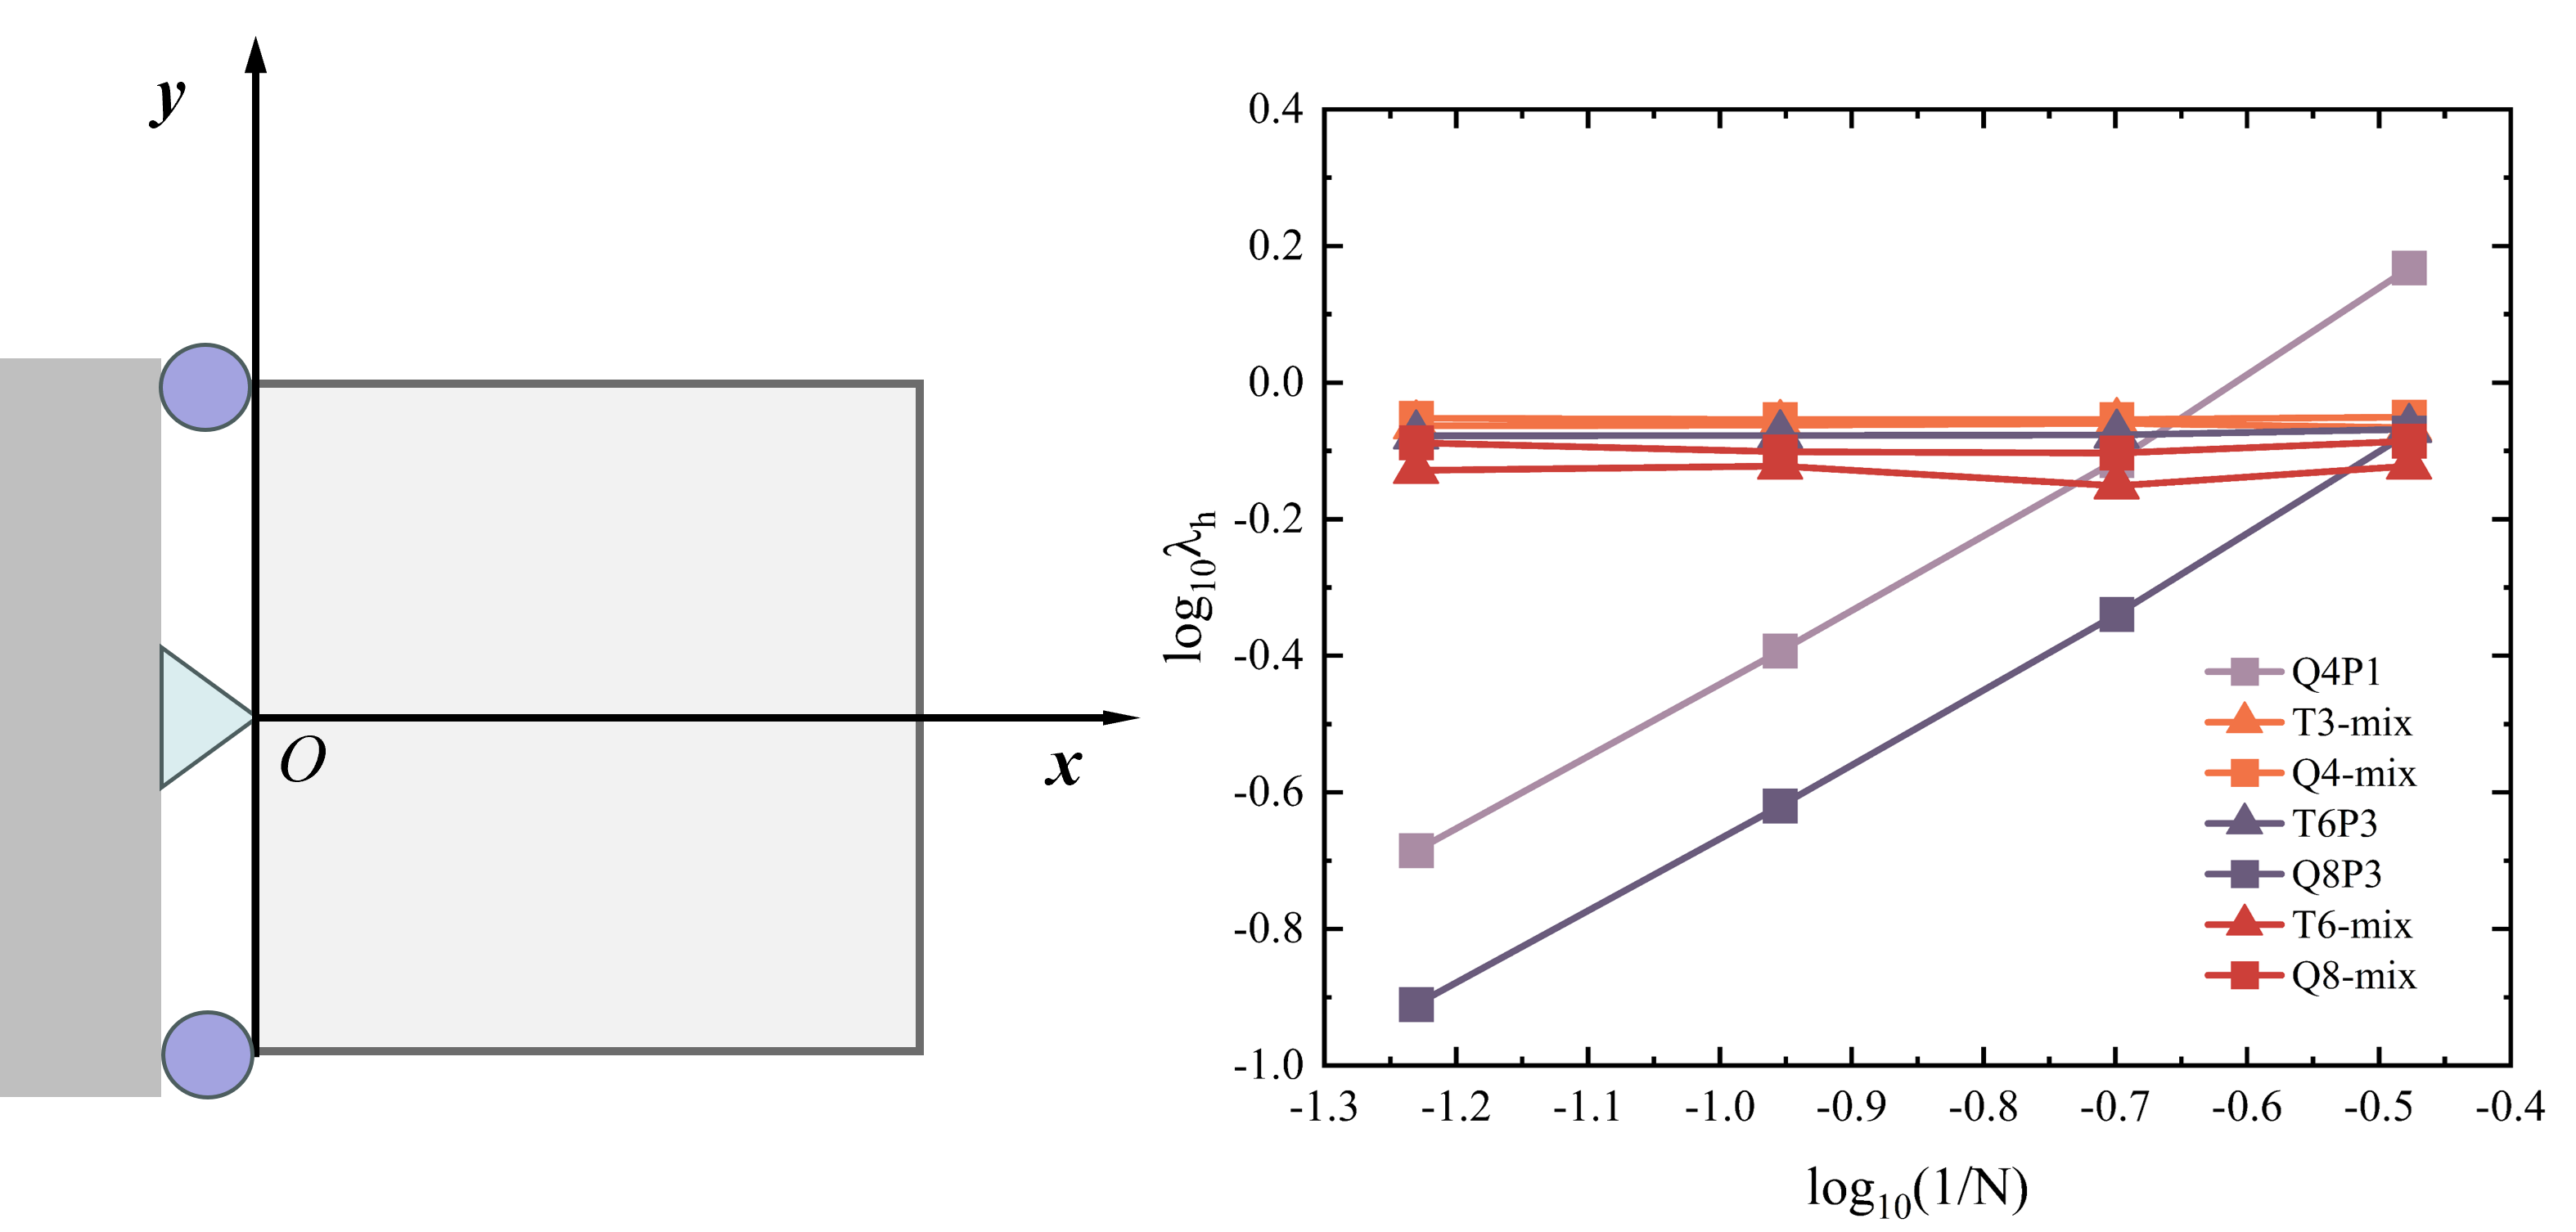
\includegraphics[width=\textwidth]{png/inf-sup.png}
\caption{Illustration of inf--sup-- and patch--tests}\label{infsup_illsutration}
\end{figure}

\subsubsection{Inf--sup test}

% \begin{figure}[!ht]
% \centering
% 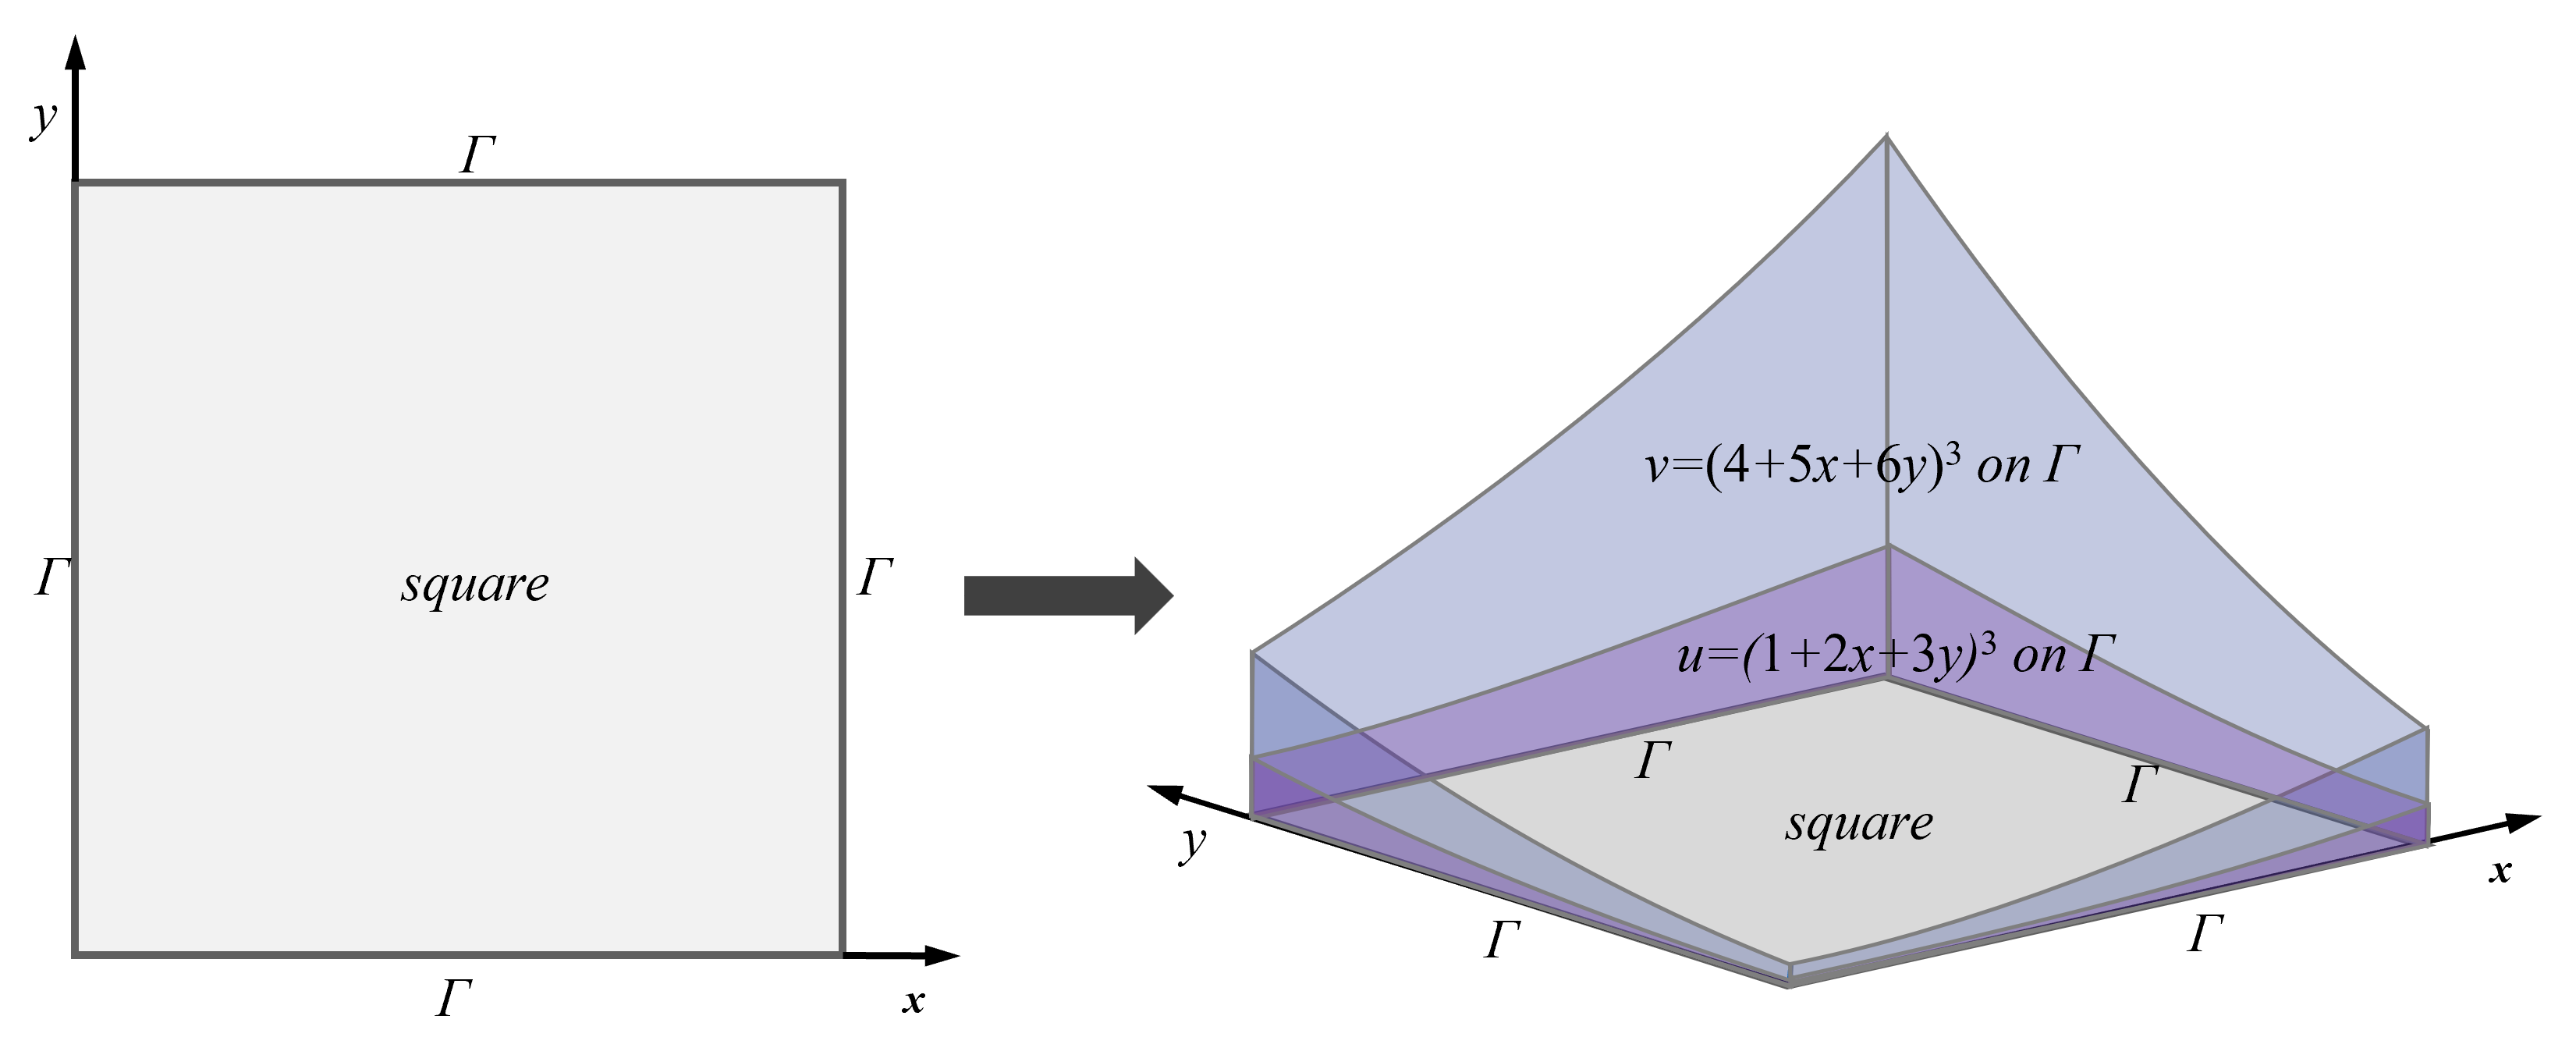
\includegraphics[width=\textwidth]{png/patchtest.png}
% \caption{Inf--sup test for various finite element formulations}\label{infsup_convergence}
% \end{figure}
% begin{figure}[!ht]
% \centering
% \includegraphics[width=\textwidth]{png/patchtest2.png}
% \caption{Inf--sup test for various finite element formulations}\label{infsup_convergence}
% \end{figure}

\begin{table}[!ht]
\centering
\caption{Results of Nearly--incompressible elasticity patch test}\label{patchtest_result}
\begin{tabular}{lcccc}
\toprule
 & \multicolumn{2}{c}{Linear patch test} & \multicolumn{2}{c}{Quadratic patch test} \\ \cline{2-5}
 & $L_2$-Error & $H_e$-Error & $L_2$-Error & $H_e$-Error \\
\midrule
    T3-stripe & & & & \\
    T3-cross & & & & \\
    T3-mix & & & & \\
    Q4 & & & & \\
    Q4R1 & & & & \\
    Q4-mix & & & \\
    T6 & & & & \\
    T6P3 & & & & \\
    T6-mix & & & & \\
    Q8 & & & & \\
    Q8P3 & & & & \\
    Q8-mix & & & & \\
\bottomrule
\end{tabular}
\end{table}

\subsection{Cantilever beam problem ?? (convergence study)}

\begin{figure}[!ht]
\centering
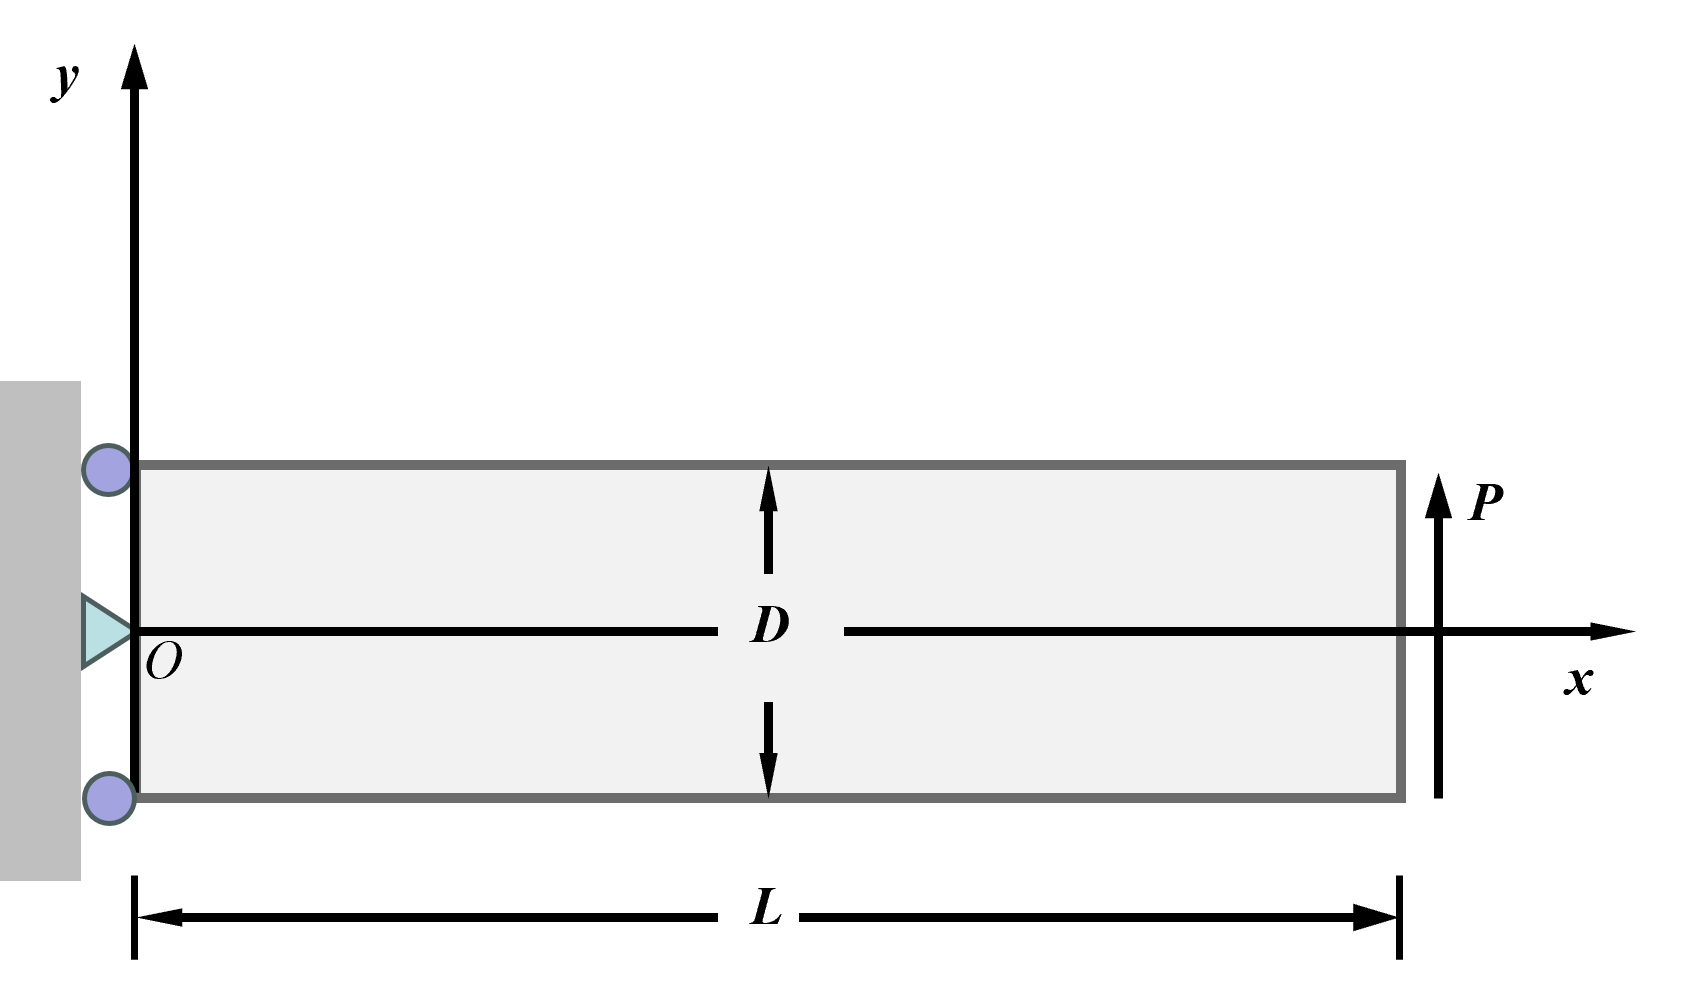
\includegraphics[width=0.6\textwidth]{png/cantilever.png}
\caption{Illustration of cantilever beam problem}\label{cantilever_illsutration}
\end{figure}

\begin{figure}[!ht]
\centering
\begin{subcaptiongroup}
% 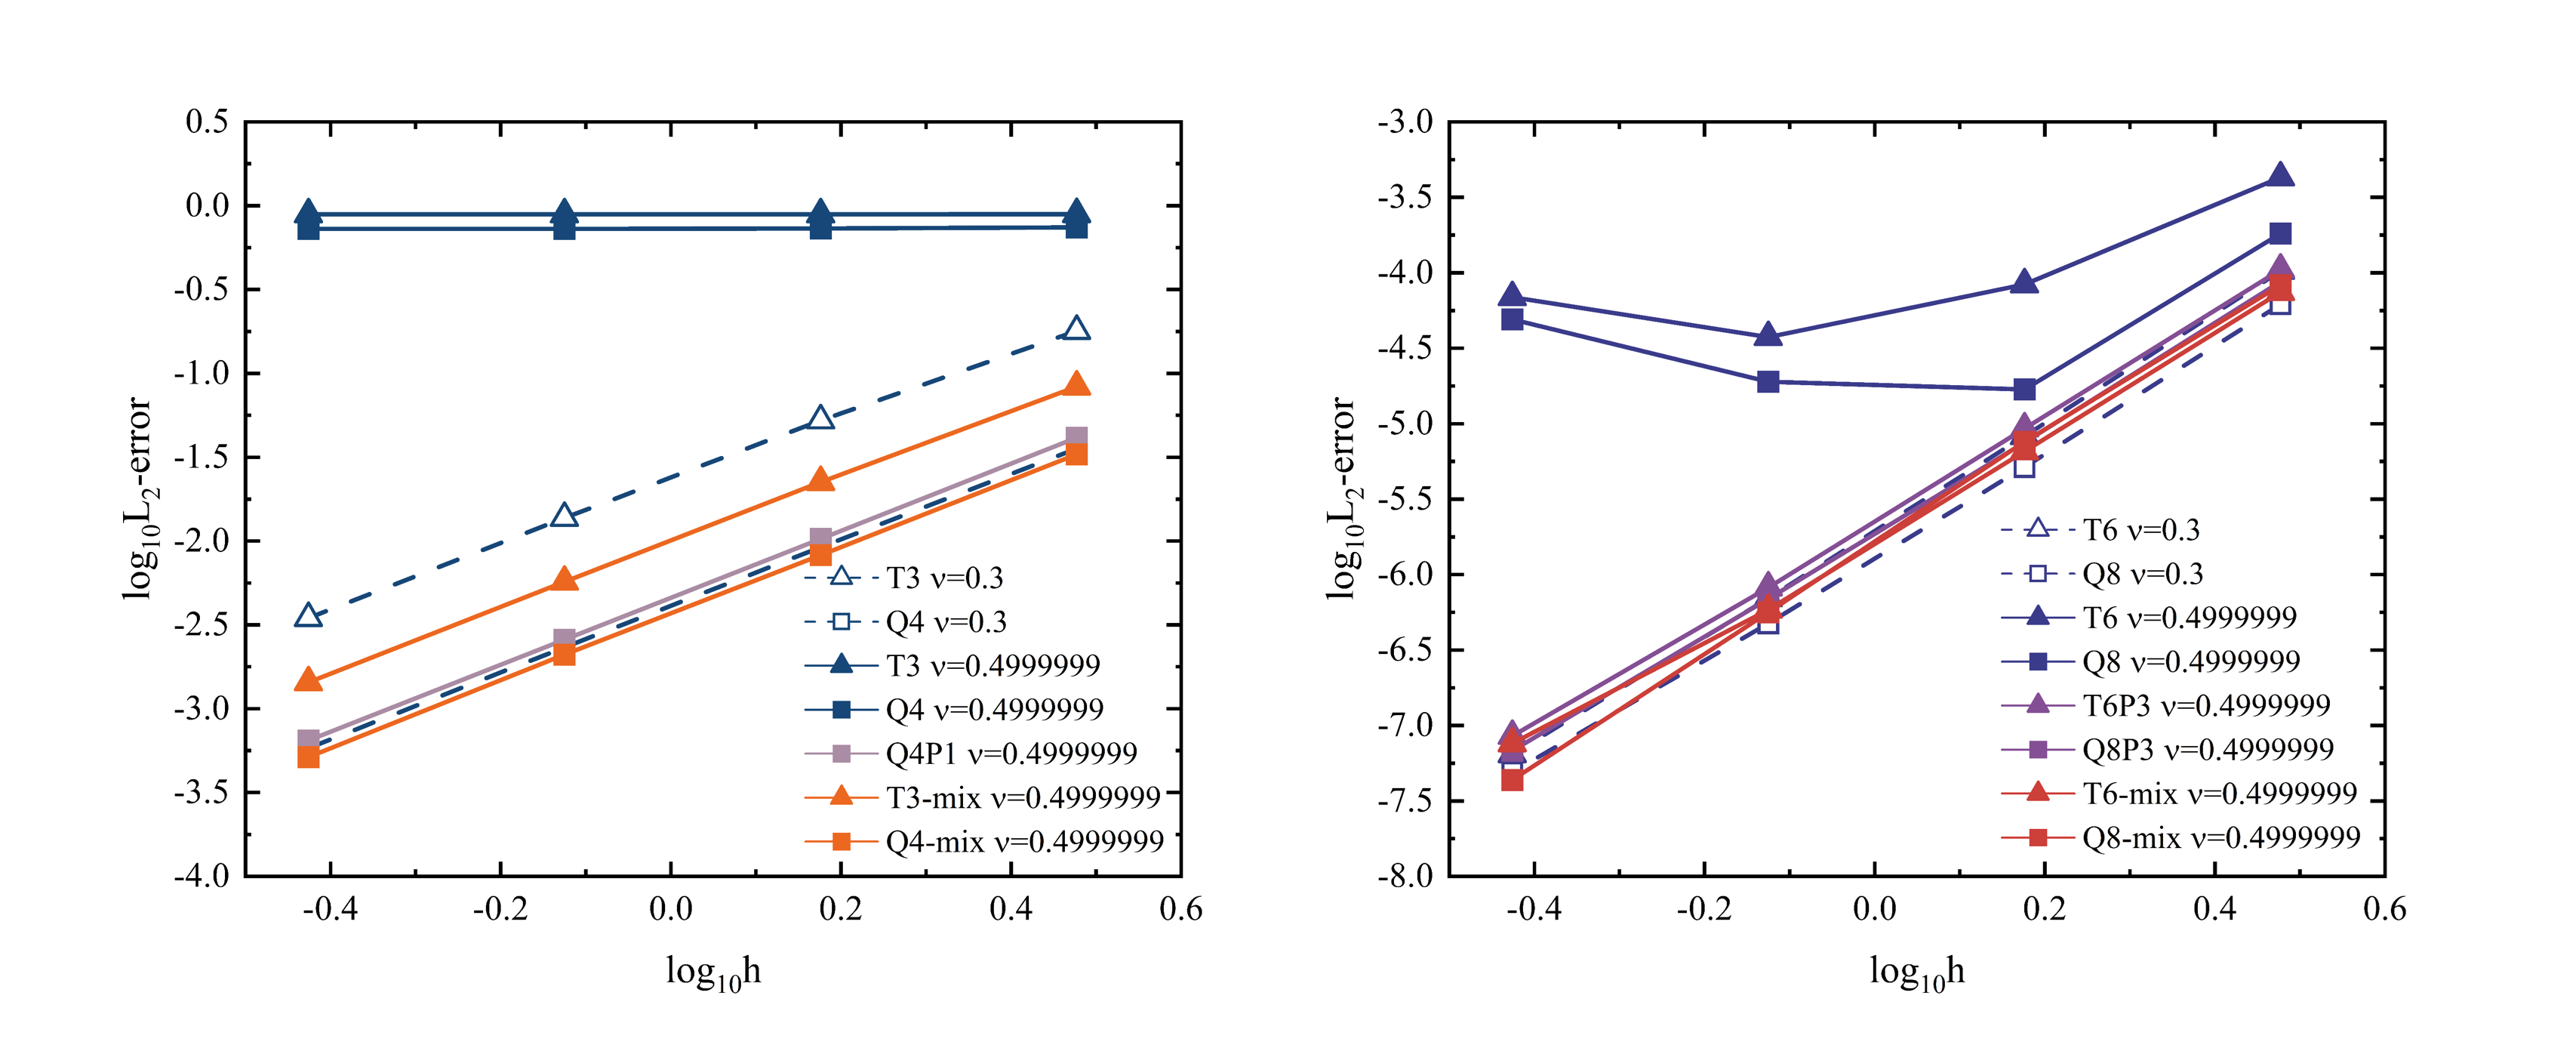
\includegraphics[width=0.49\textwidth]{png/cantilever2.png}
%     \phantomcaption\label{cantilever_l2}
% 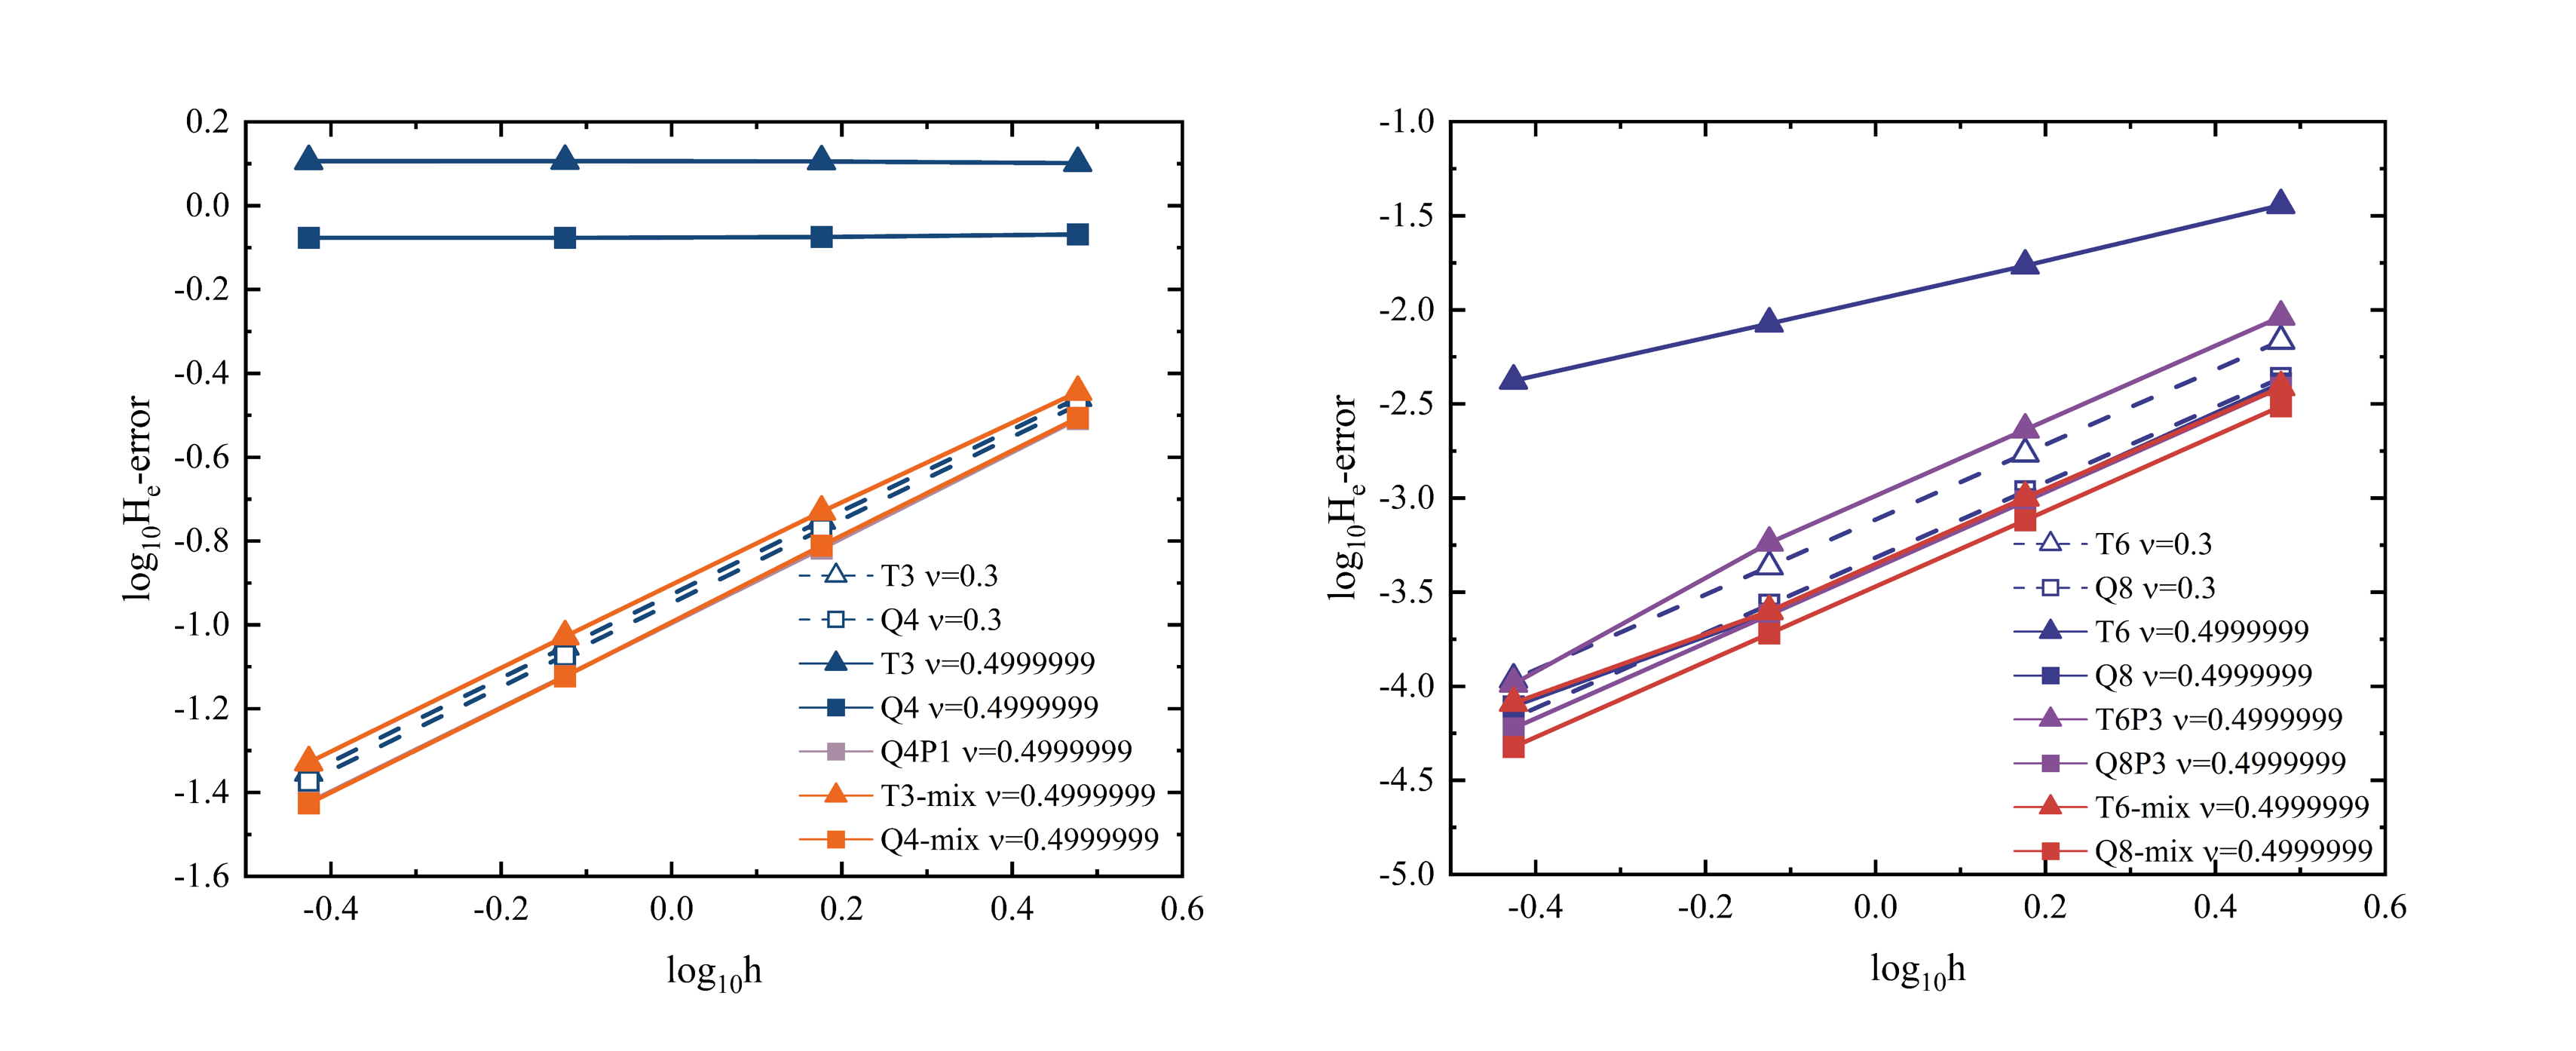
\includegraphics[width=0.49\textwidth]{png/cantilever3.png}
%     \phantomcaption\label{cantilever_h1}
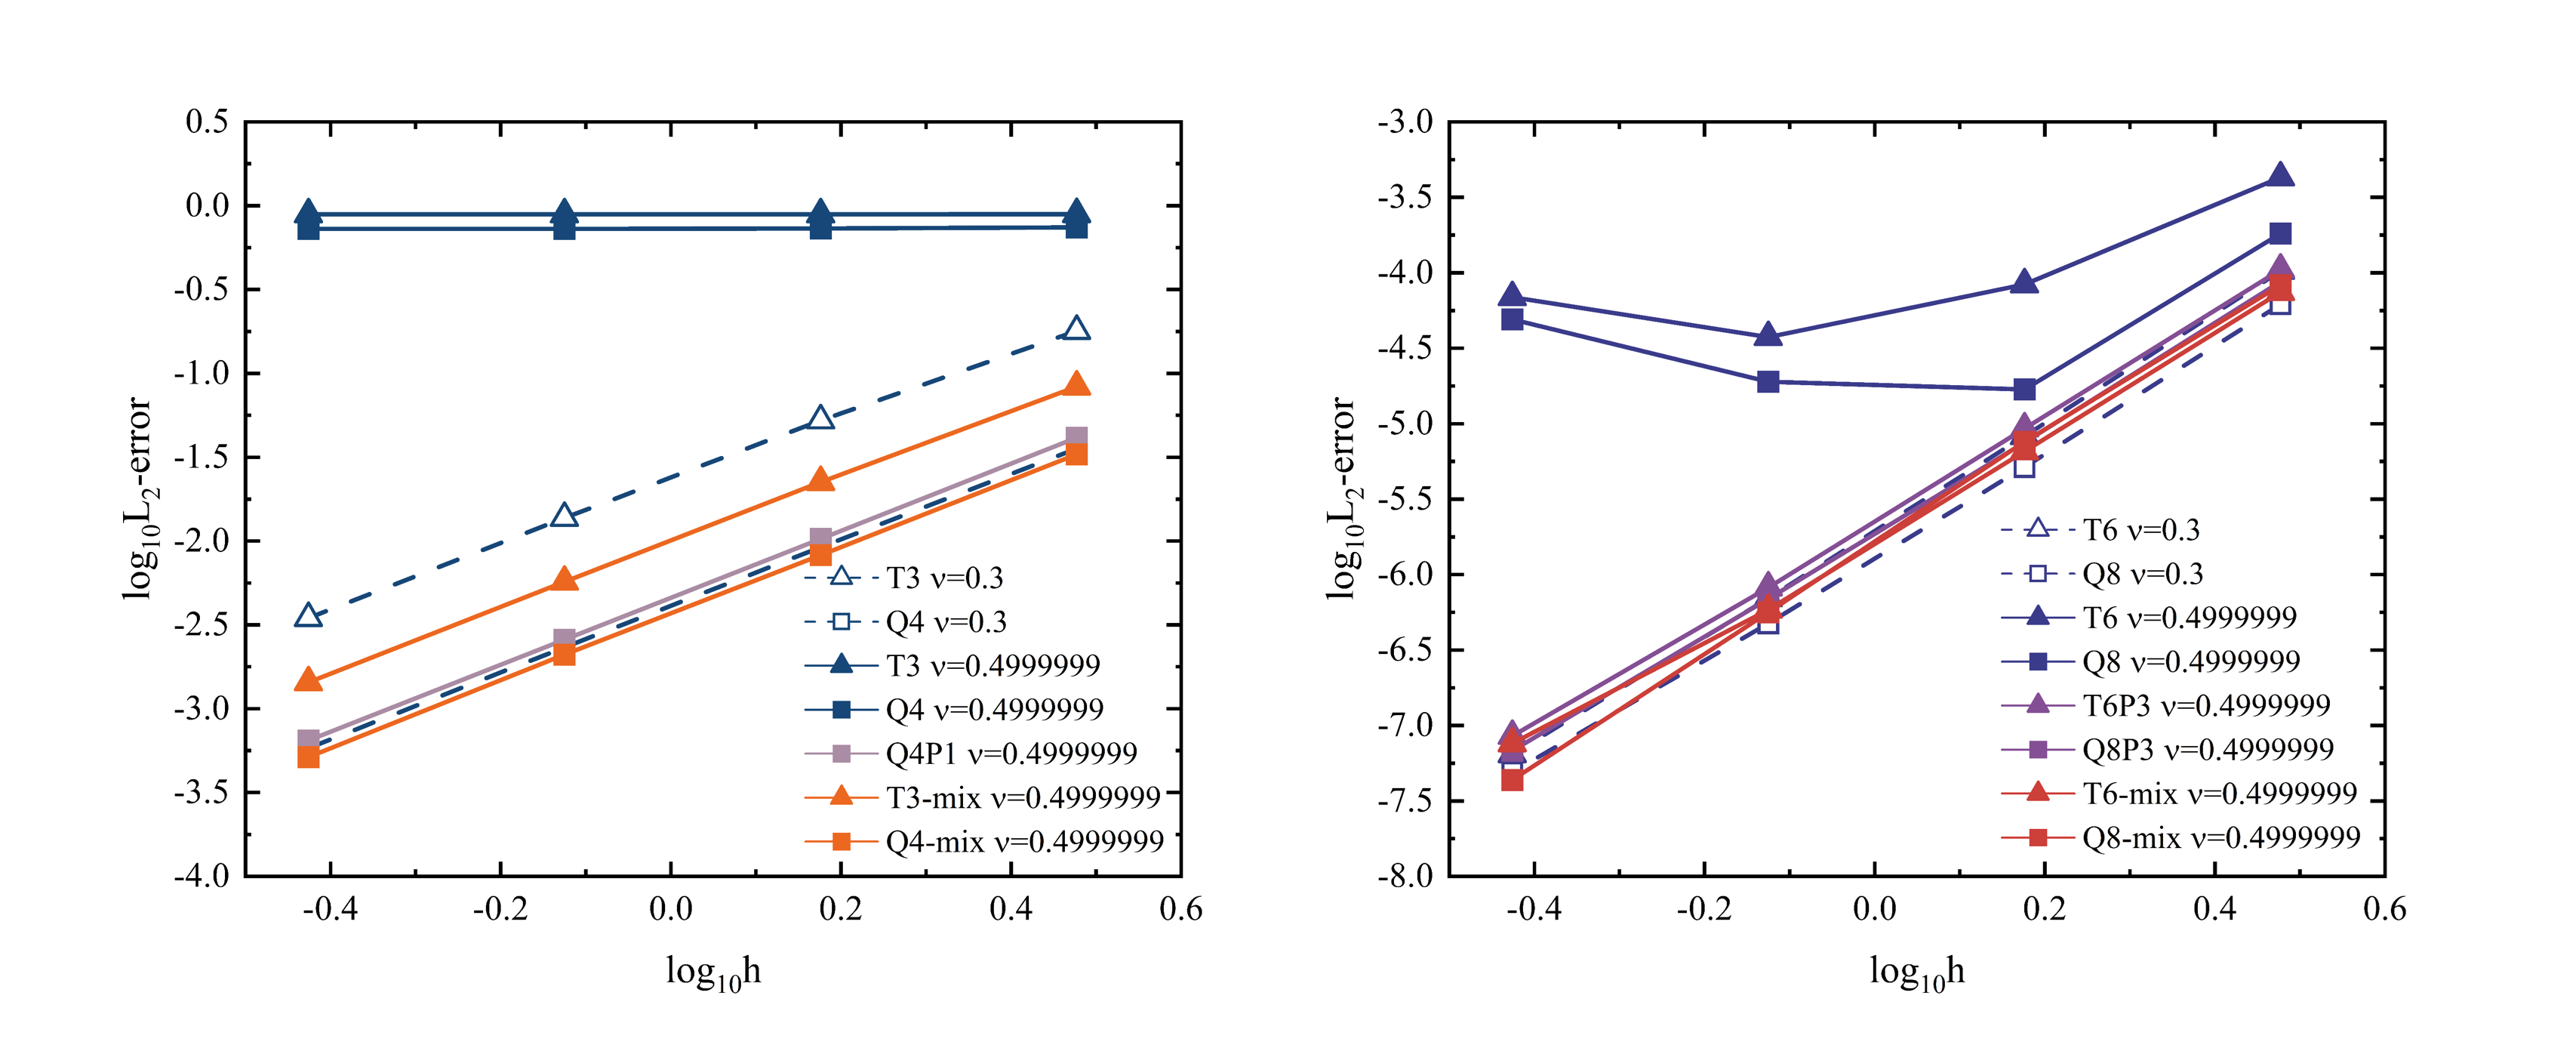
\includegraphics[width=\textwidth]{png/cantilever2.png}
    \phantomcaption\label{cantilever_l2}
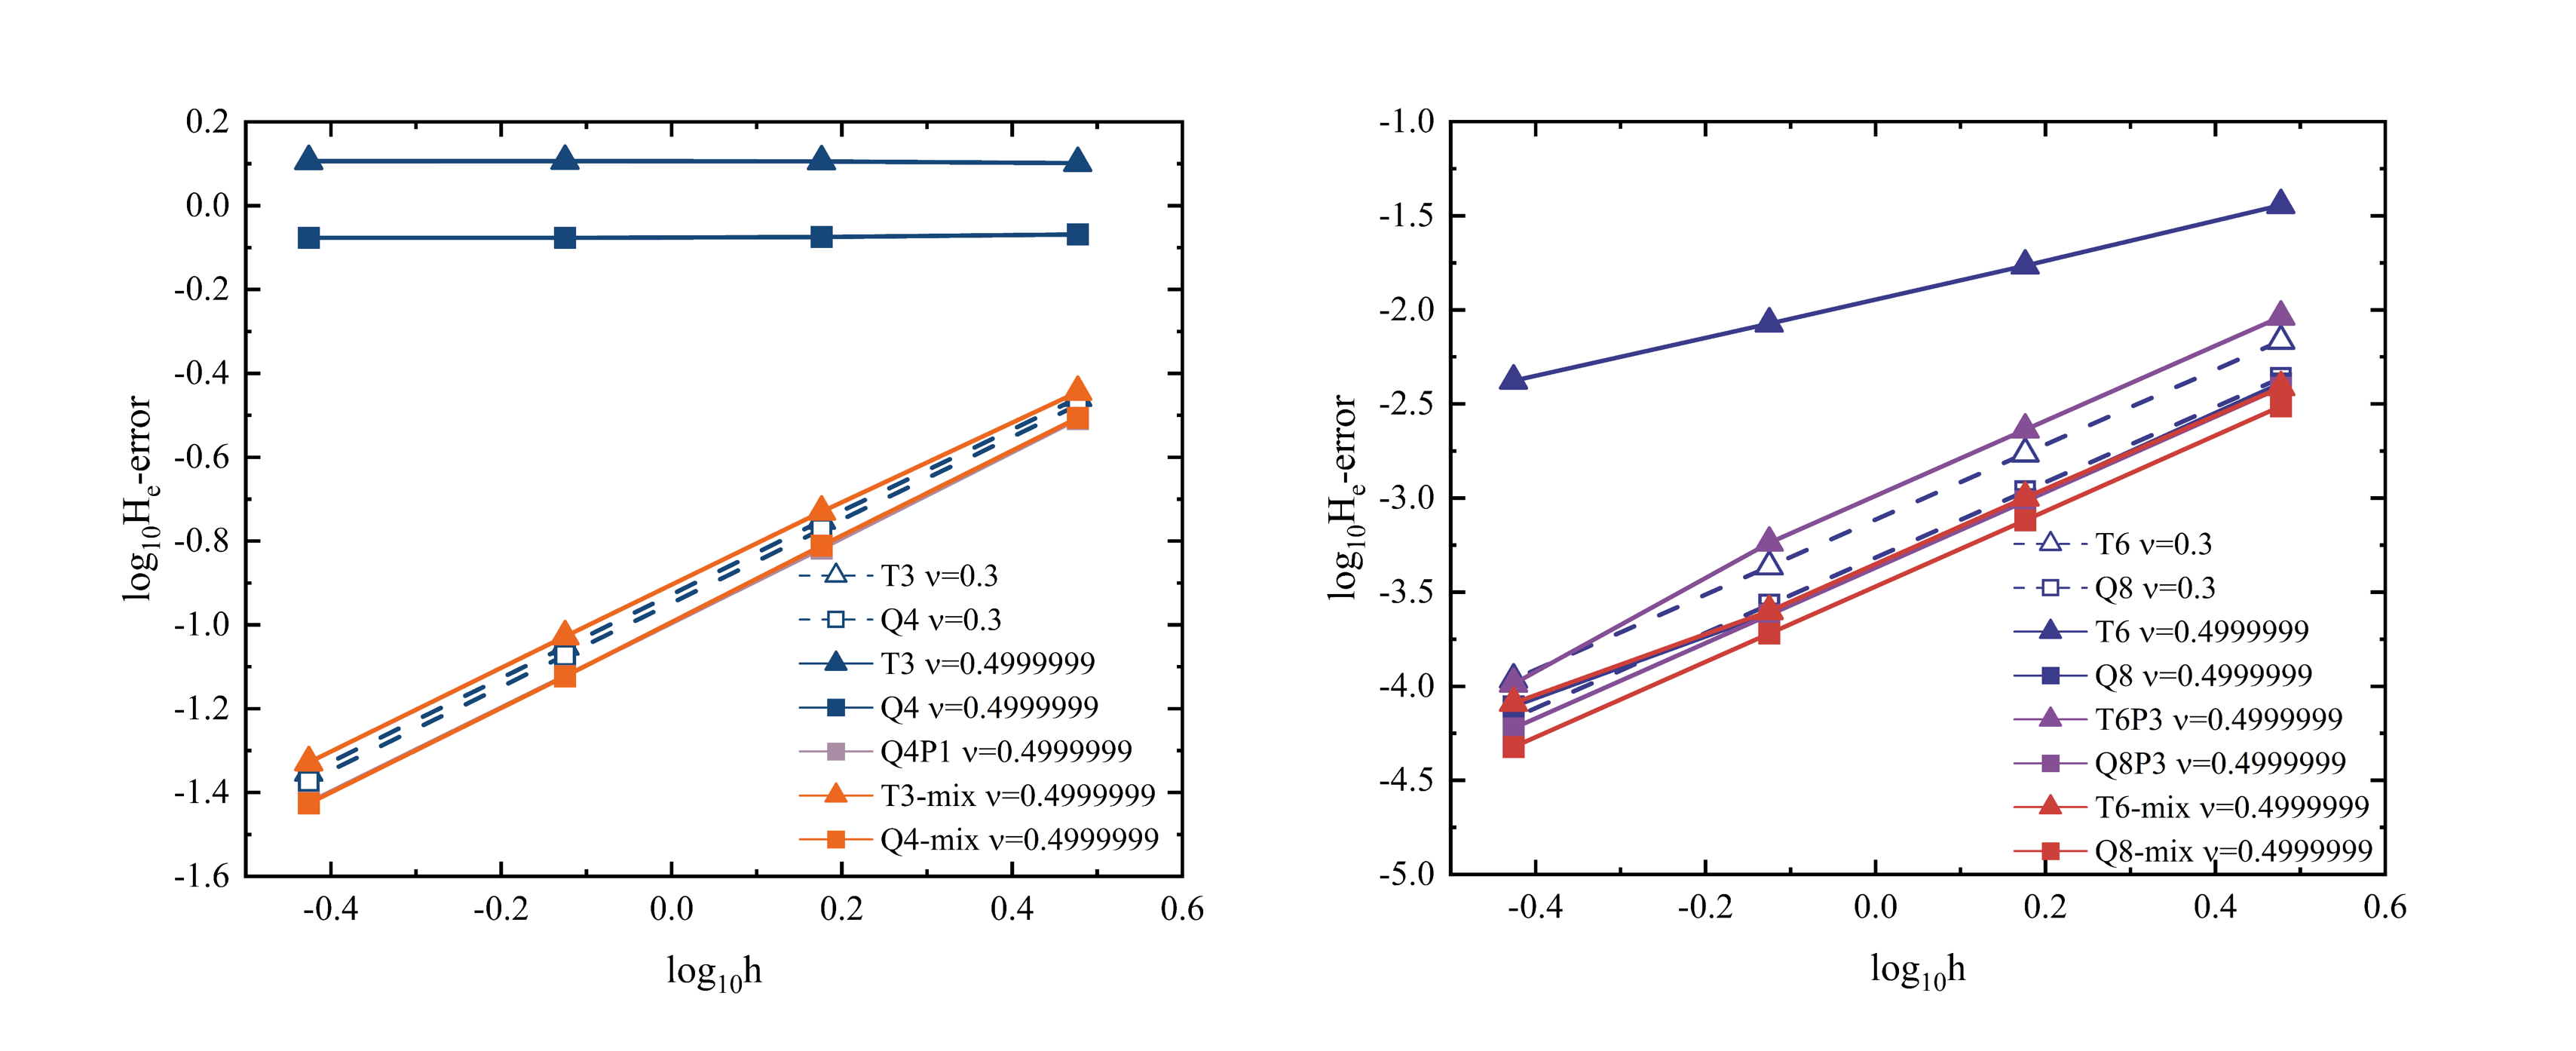
\includegraphics[width=\textwidth]{png/cantilever3.png}
    \phantomcaption\label{cantilever_h1}
\end{subcaptiongroup}
\caption{Convergence comparison of cantilever beam problem: \subref{cantilever_l2} $L^2$-Error; \subref{cantilever_h1} $H^e$-Error}\label{cantilever_illsutration}
\end{figure}

\begin{figure}[!ht]
\centering
% \includegraphics[width=\textwidth]{png/cantilever4.png}
\caption{Contour plots of cantilever beam problem}\label{cantilever_contour}
\end{figure}

\subsection{Cook membrane problem}

\begin{figure}[!ht]
\centering
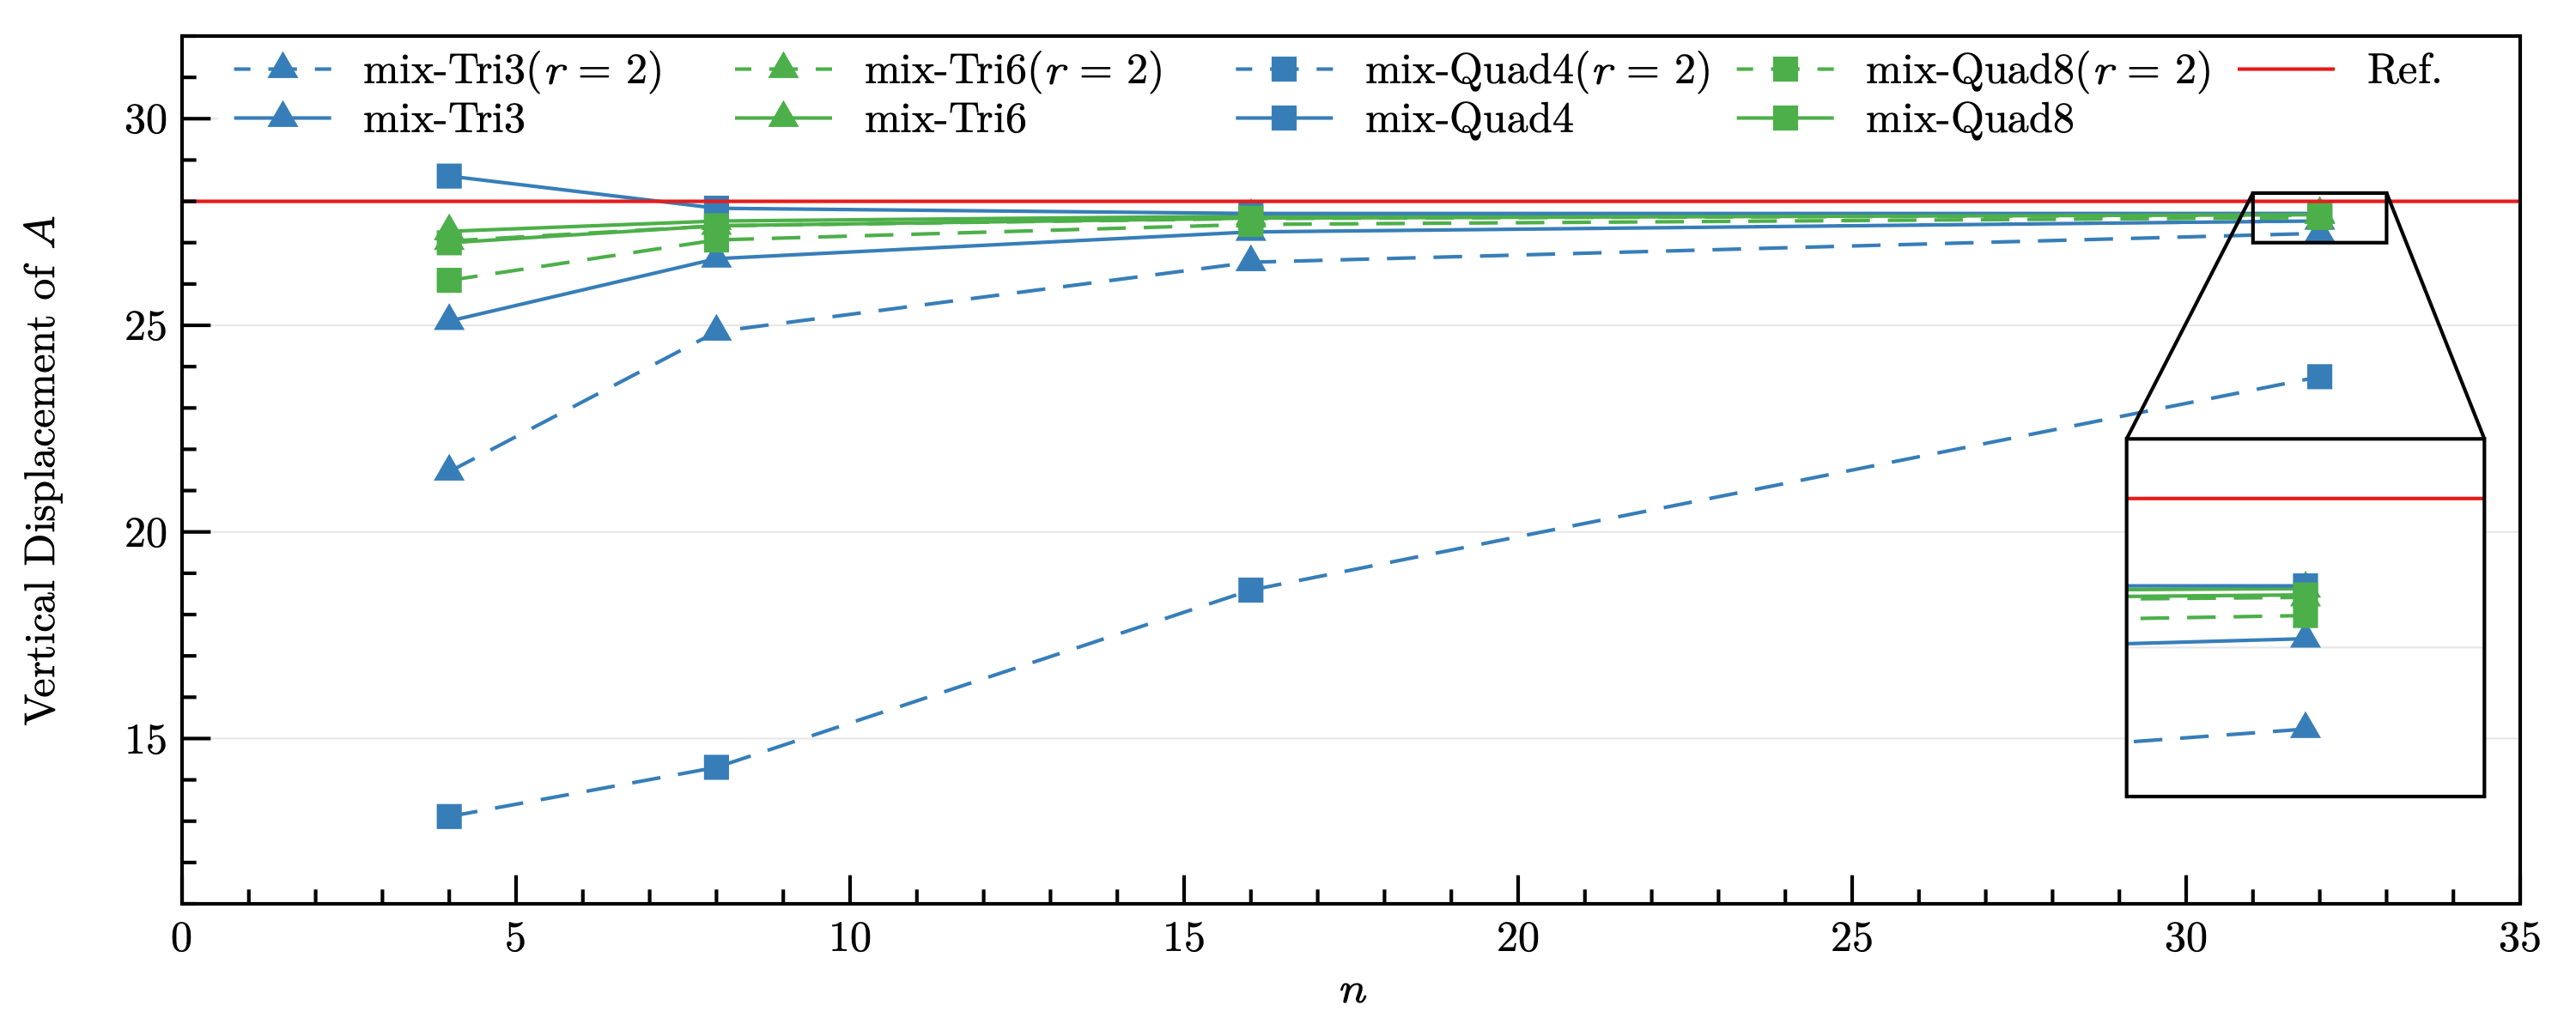
\includegraphics[width=0.6\textwidth]{png/cook.png}
\caption{Illustration of cook membrane problem}\label{cook_illsutration}
\end{figure}

\begin{figure}[!ht]
\centering
\includegraphics[width=0.7\textwidth]{png/cook2.png}
\caption{Convergence comparison of cook membrane problem}\label{cook_convergence}
\end{figure}

\begin{figure}[!ht]
\centering
% \includegraphics[width=\textwidth]{png/cook3.png}
\caption{Contour plots of cook membrane problem}\label{cook_contour}
\end{figure}

\subsection{Block under compression problem}
Problem reference \cite{reese2000}, Neo-Hooke model, T4 and Q8 elements.

\begin{figure}[!ht]
\centering
% \includegraphics[width=\textwidth]{}
\caption{Illustration of block under compression problem}\label{block_illsutration}
\end{figure}

\begin{figure}[!ht]
\centering
% \includegraphics[width=\textwidth]{}
\caption{Convergence comparison of block under compression problem}\label{block_convergence}
\end{figure}

\begin{figure}[!ht]
\centering
% \includegraphics[width=\textwidth]{}
\caption{Contour plots of block under compression problem}\label{block_contour}
\end{figure}
